\section{Problème 1D}

En repartant de~\eqref{dgm:to_solve} et en considérant un problème 1D (voir figure~\ref{fig:FEM:propa_1D}), il vient :

\begin{equation}
    \int_{\partial\Omega}\ul{v}^T\uul{A}\ul{u}\dd\Gamma = 0 \Leftrightarrow
\underbrace{\ul{v}^T(L)\uul{A}\ul{u}(L)}_\mathrm{droite} - \underbrace{\ul{v}^T(0)\uul{A}\ul{u}(0)}_\mathrm{gauche}
\quad,\quad \forall\ul{v}\label{dgm:d_g}
\end{equation}

\subsection{Condition limite à droite}

A droite, la paroi rigide implique :

\begin{eqnarray*}
    v(L) = 0 & \Leftrightarrow &
    \begin{pmatrix}
        1 & 0
    \end{pmatrix}
    \begin{pmatrix}
        v\\p
    \end{pmatrix}
     = 0\\
    & \Leftrightarrow &
    \begin{pmatrix}
        1 & 0
    \end{pmatrix}
    \begin{bmatrix}
        1 & 1\\
        Z_0 & -Z_0
    \end{bmatrix}
    \begin{pmatrix}
        \tilde{u}^+\\\tilde{u}^-
    \end{pmatrix}\\
    & \Leftrightarrow &
    \tilde{u}^+ = -\tilde{u}^- \Leftrightarrow \tilde{u}^+ = R^-\tilde{u}^-
\end{eqnarray*}

En utilisant maintenant~\eqref{dgm:sep_u}, et en réutilisant le résultat précédent :

\begin{eqnarray}
    \ul{u} = \ul{P}^+\tilde{u}^+ + \ul{P}^-\tilde{u}^-
        & \Leftrightarrow & \ul{u} = \ul{P}^+\tilde{u}^+ + \ul{P}^-R^-\tilde{u}^+\notag\\
        & \Leftrightarrow & \ul{u} = \left(\ul{P}^+ + \ul{P}^-R^-\right)\ul{Q}^+u\label{dgm:droite}
\end{eqnarray}

\subsection{Condition limite à gauche}

A gauche, les conditions de continuité impliquent :

\begin{figure}[!ht]
	\centering
	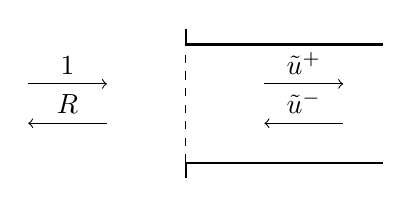
\begin{tikzpicture}
    \draw[thick] (0,-.2) -- (0,0) -- (2.5,0);
    \draw[thick] (0,1.7) -- (0,1.5) -- (2.5,1.5);

    \draw[dashed] (0,0) -- (0,1.5);

    \draw[->] (-2,1) -- ++(1,0) node[midway,above] {$1$};
    \draw[->] (-1,.5) -- ++(-1,0) node[midway,above] {$R$};
    \draw[->] (1,1) -- ++(1,0) node[midway,above] {$\tilde{u}^+$};
    \draw[->] (2,.5) -- ++(-1,0) node[midway,above] {$\tilde{u}^-$};
\end{tikzpicture}


    \caption{\label{fig:interface}Interface à gauche du problème.}
\end{figure}

\begin{equation*}
    \begin{array}{c}
        P\begin{Bmatrix}1\\R\end{Bmatrix} = P\begin{Bmatrix}\tilde{u}^+\\\tilde{u}^-\end{Bmatrix}\\
            \Leftrightarrow \left\{\begin{array}{l}
                    \tilde{u}^+ = 1\\
                    \tilde{u}^- = R = \ul{Q}^-\ul{u}
            \end{array}\right.
    \end{array}
\end{equation*}

En ré-exprimant $u$, il vient :

\begin{equation}
    \ul{u} = \ul{P}^+\tilde{u}^+ + \ul{P}^-\tilde{u}^- \Leftrightarrow \ul{u} = \ul{P}^+ + \ul{P}^-\ul{Q}^-\ul{u}\label{dgm:gauche}
\end{equation}

En remettant~\eqref{dgm:droite} et~\eqref{dgm:gauche} dans~\eqref{dgm:d_g} et en utilisant les expressions discrétisées
des champs, il vient :

\begin{equation}
    \begin{array}{rcl}
        \GV^T\bigg[\uul{U}_v^T(L)\uul{P\Lambda Q}\left(\ul{P}^+ + \ul{P}^-R^-\right)\ul{Q}^+\uul{U}_u(L) & - &
    \uul{U}_u(0)\uul{P\Lambda Q}\ul{P}^-\ul{Q}^-\uul{U}_u(0)\bigg] \GU\\
    & = & \GV^T\uul{U}_v^T(0)\uul{P\Lambda Q}\ul{P}^+ \quad,\quad \forall\GV
    \end{array}
\end{equation}

L'équation précédente étant valable pour tout vecteur $\GV$ il est possible de supprimer ce terme.
La solution pour $\GU$ est alors calculable par simple division matricielle.

\subsection{Simulation}

En 1D, la DGM avec ondes planes présentée ici conduit à une solution exacte. Pour cette simulation, plutôt que l'analyse
de la convergence pour le calcul du coefficient, c'est le tracé du profil de pression qui est réalisé. Le résultat est
présenté en figure~\ref{fig:dgm:simul}.

\begin{figure}[!ht]
    \centering
    \includegraphics[width=11cm]{part2/figs/comp_hermiteFEM_dgm.png}
    \caption{\label{fig:dgm:simul}En haut : profil de pression dans la cavité par méthode de Galerkin discontinue (en rouge) et
    profil de référence (en bleu). En bas : erreur relative (norme $L_2$ des pressions) pour chaque point.}
\end{figure}

Aucune différence n'est visuellement constatable entre les deux courbes. Qui plus est, l'erreur, à presque $10^{-13}$,
s'approche du bruit numérique.
